\documentclass[a4paper,12pt]{article}
\usepackage[utf8]{inputenc}
\usepackage{graphicx}
\usepackage{amsmath}
\usepackage{float}
\usepackage{parskip}

\usepackage[style=apa]{biblatex}
\addbibresource{inquiry.bib}

% TODO: 833 words

\usepackage{hyperref}

\title{How has COVID impacted economic activity and what have been the extent of these impacts?}
\author{Terry Qi}

\begin{document}

\maketitle

Word count: 797

Article: https://www.bbc.com/news/business-54186359, Covid pushes New Zealand into worst recession in years, 17/09/2020, published by the BBC, on 17/09/2020, accessed 27/10/2021

Topic: Macroeconomics

Key Concept: Change

\newpage
\section*{Article}

\textit{New Zealand is in its deepest recession in decades, following strict measures in response to the Covid-19 pandemic which were widely praised.}

The country's GDP shrank by 12.2\% between April and June as the lockdown and border closures hit.

It is New Zealand's first recession since the global financial crisis and its worst since 1987, when the current system of measurement began.

But the government hopes its pandemic response will lead to a quick recovery.

The nation of nearly five million was briefly declared virus free, and although it still has a handful of cases, it has only had 25 deaths.

The economy is likely to be a key issue in next month's election, which was delayed after an unexpected spike in Covid-19 cases in August.

Stats NZ spokesman Paul Pascoe said the measures implemented since 19 March have had a huge impact of some sectors of the economy.

"Industries like retail, accommodation and restaurants, and transport saw significant declines in production because they were most directly affected by the international travel ban and strict nationwide lockdown," he said.

Prime Minister Jacinda Ardern's government has said the success in suppressing the virus is likely to help recovery prospects.

Finance Minister Grant Robertson said the GDP numbers were better than expected, and suggested a strong recovery ahead.

"Going hard and early means that we can come back faster and stronger," he said.

Some economists are also predicting a swift recovery, because of New Zealand's strong response to the virus.

"We expect the June quarter's record-breaking GDP decline to be followed by a record-breaking rise in the September quarter," said Westpac Senior Economist Michael Gordon.

Ms Ardern said she backs the economy's ability to rebound.

"I think one of the key questions here is not just about what's happened over that June quarter in terms of the effect of lockdown. It's actually about the rebound - and I back New Zealand's rebound," she said.

Ms Ardern said activity is already picking up as the country has been able to open up a lot more quickly compared with other nations.

"Even with some of the more recent restrictions, we've seen a return to activity, whereas compared to Australia we are in a much better position," she added.

However Treasury forecasts released yesterday suggested massive debt and continuing disruptions are likely to delay a full recovery.

The opposition National party accused the government of a lack of pragmatism that made the impact worse than it needed to be.

New Zealand recorded a steeper drop than neighbouring Australia, where the lockdown was less severe.

But the state of Victoria has faced a second lockdown, which is likely to weigh on Australia's economic recovery.

\newpage
% planning
% gdp shrank 12.2% lockdown. first recession. impact on retail, accommodation, restaurations, transport, decline production travel bans.

% more research: inflation, unemployment, imports & exports, economic growth



% unemployment, suddenly peeked at 5.3% in third quarter of 2020, slowly growing in the first two quarters of the pandemic

% inflation, slowly increasing from the third quarter of  2019, decreases at the 2nd quarter in 2020.

% imports & exports, third quarter: goods exports decreased, imports increases; service net exports are negative in second quarter

% economic growth: GDP growth is negative from the third quarter, recovering at next year second quarter


% https://www.stats.govt.nz/information-releases/balance-of-payments-and-international-investment-position-june-2021-quarter
% https://www.stats.govt.nz/information-releases/consumers-price-index-september-2021-quarter
% https://www.stats.govt.nz/information-releases/labour-market-statistics-june-2021-quarter
% https://www.stats.govt.nz/indicators/gross-domestic-product-gdp

% https://www.stats.govt.nz/news/household-saving-falls-in-the-march-2021-quarter#:~:text=The%20household%20saving%20ratio%2C%20which,in%20the%20December%202020%20quarter.&text=Net%20disposable%20income%20represents%20the,accounting%20for%20things%20like%20taxes.

\section*{Topic}
The article chosen discusses the impact of COVID-19 upon New Zealand's economy in 2020. It  measured a 12.2\% decrease in the national nominal GDP, stating a deep recession. This discussion will focus on the \textbf{change} in the retail sectors of the economy upon COVID through the application of economic theory, and will evaluate its impacts on the wider economy.

\section*{Theory}
Aggregate demand (AD), is defined as the summation of all the market demands --- $AD = C+I+G+(X-M)$. As stated in the article, the pandemic had directly affected the retail industry through a decrease in production quantity. This is likely caused by the various international travel bans and strict nationwide lockdowns, restricting the demand from consumers, and directly decreasing the consumption component of AD.

The Keynsian model of the economy is used, for NZ have strong labor unions and regulations \parencite{labor}, creating sticky wages as price levels decreases, fulfilling the assumptions of the Keynsian model. Additionally, the initial level of real output ($Y_1$) is drawn close to the level of full employment ($Y_f$), for average unemployment rates in the NZ is relatively low at around 4\% throughout 2020 \parencite{unemploy}, thus lessening the recessionary gap of size $Y_f-Y_1$.

This is shown in figure \ref{fig:asad} through a leftwards shift of the aggregate demand from $AD_1$ to $AD_2$, which reduces the NZ real GDP (real output) for total expenditure and money flow will slow down from a lack of demand to do so, reducing real GDP from $Y_1$ to $Y_2$. Moreover, the small recessionary gap means that a moderate decrease in the price level, from $PL_1$ to $PL_2$, is to be expected, as the decrease in real output creates vacancies in the demand of factors of productions, causing their owners to lower their cost/interest rates to maximize profit, thus lowering the cost of production and decreasing the price level.

% TODO: put on top
% theory
\begin{figure}[H]
    \centering
    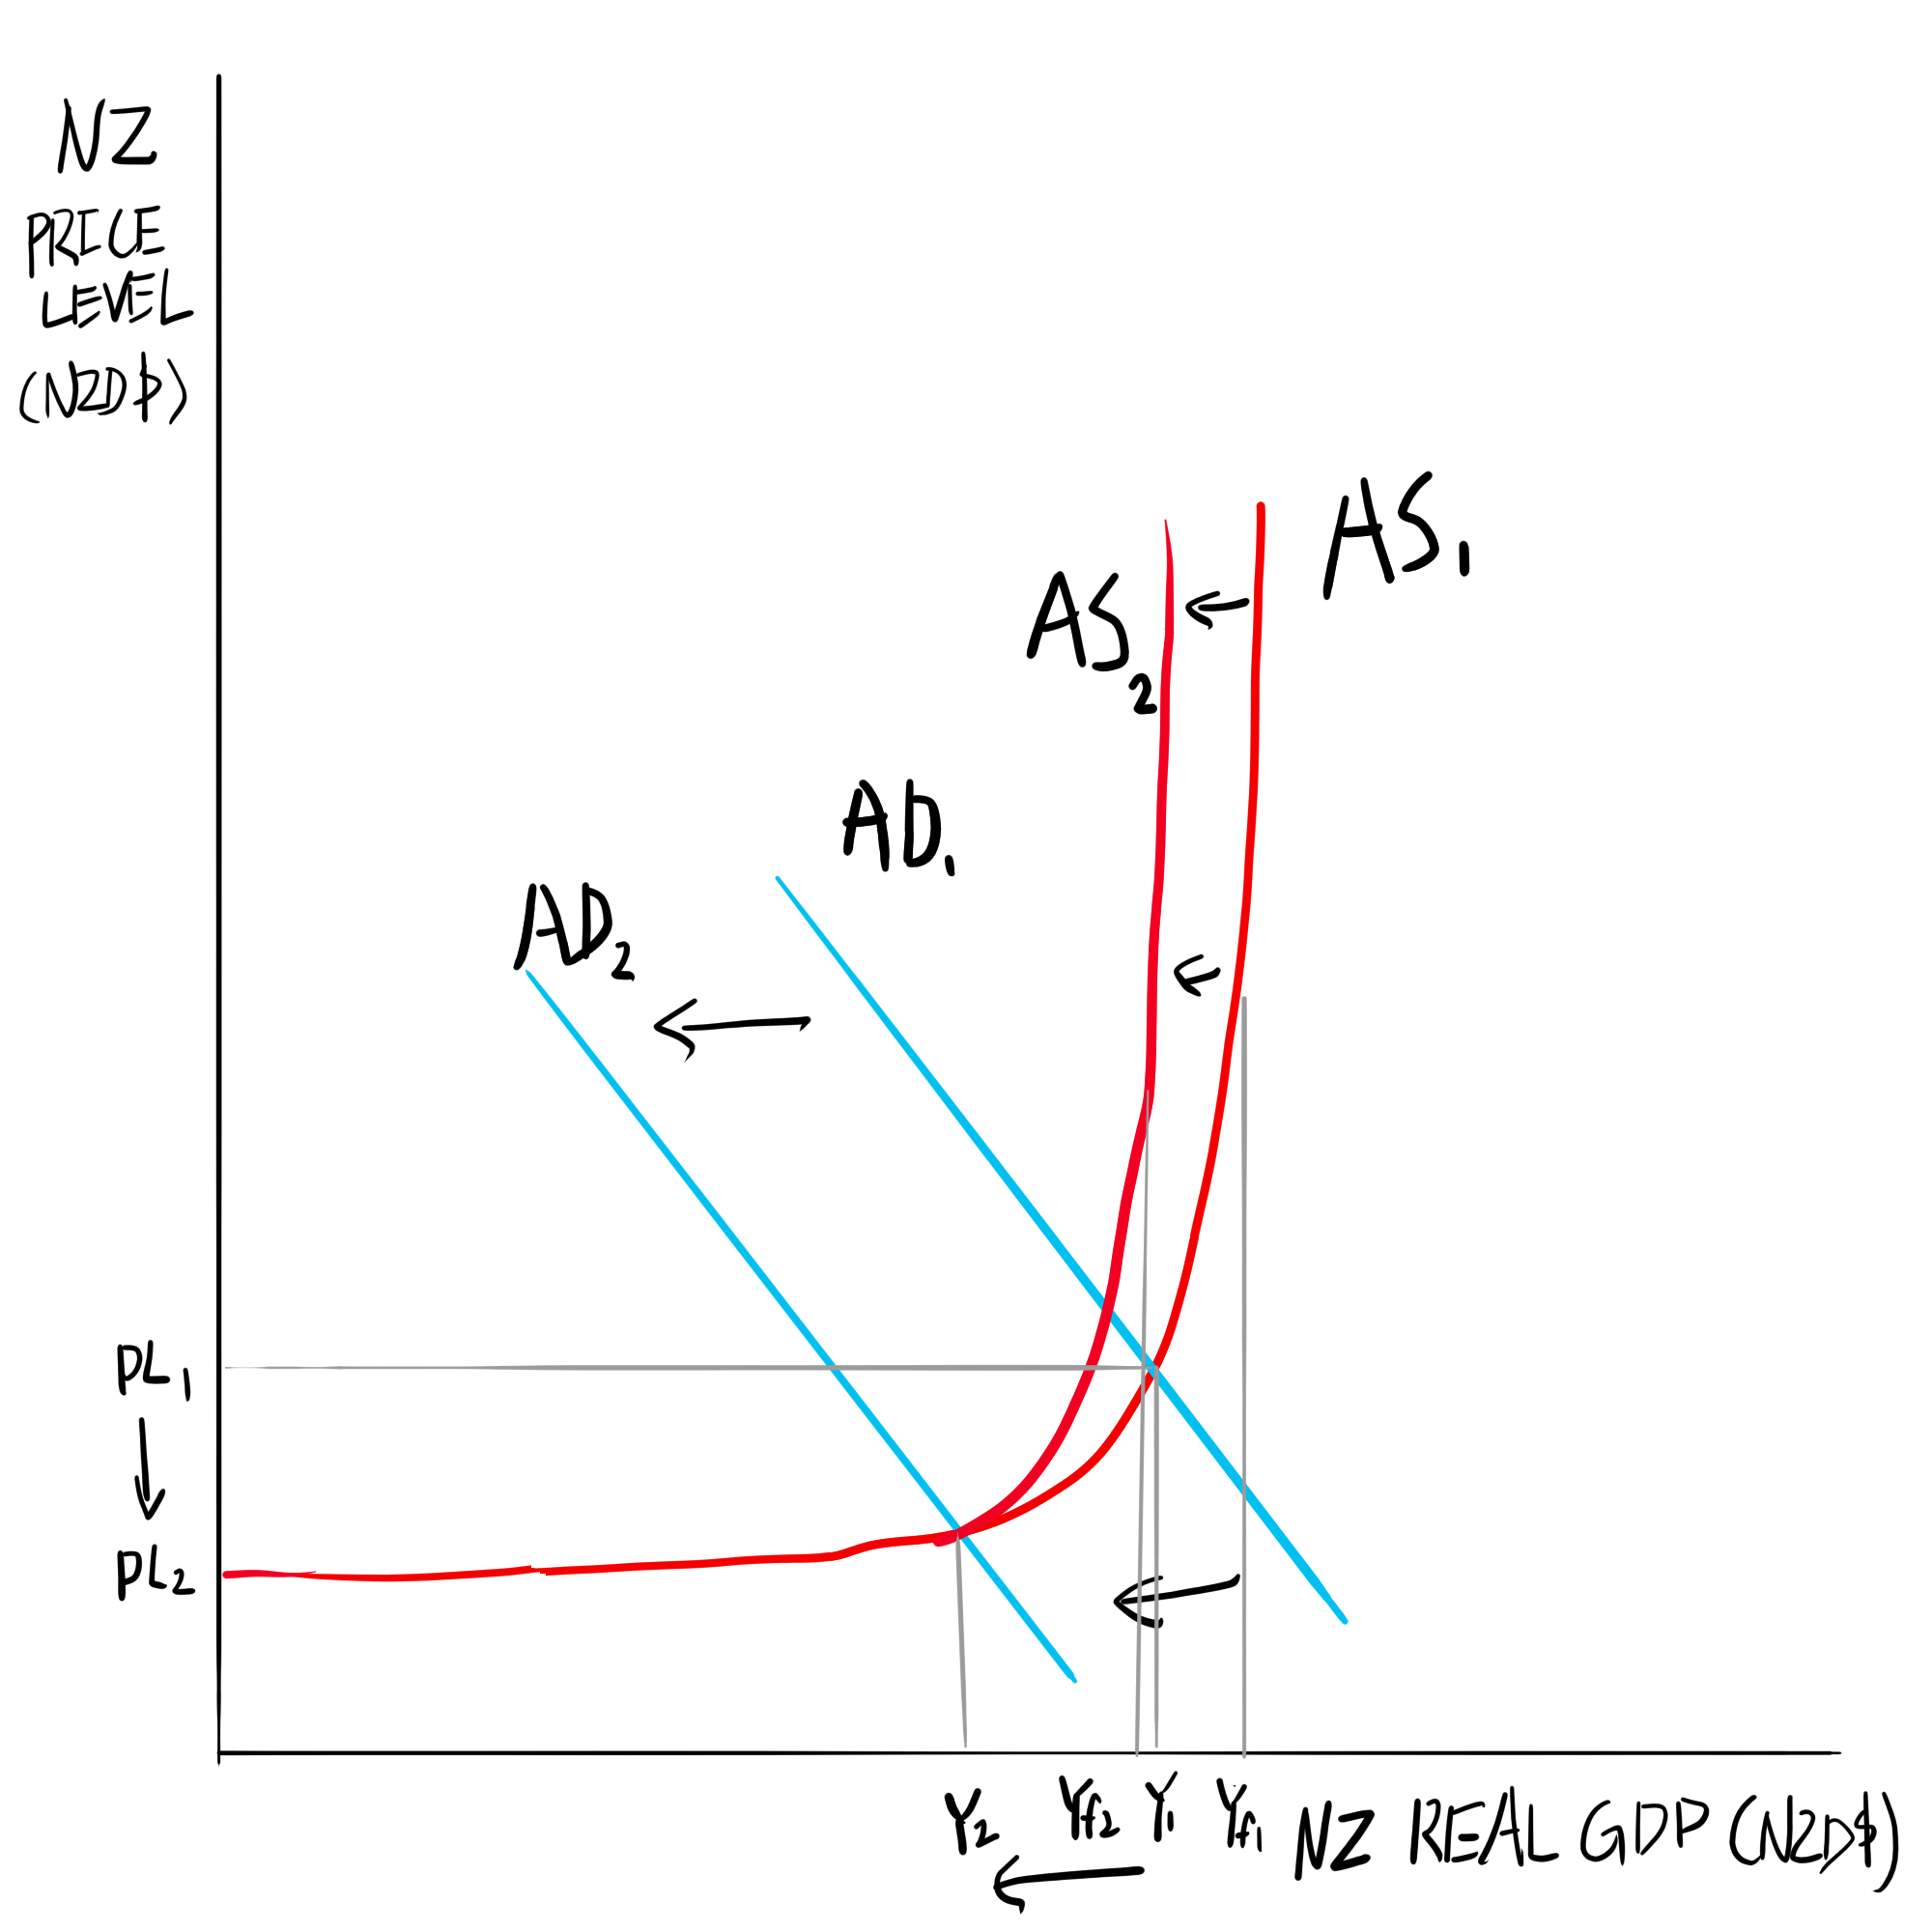
\includegraphics[scale=0.6]{assets/asad.png}
    \caption{NZ AD/AS diagram during COVID}
    \label{fig:asad}
\end{figure}

Furthermore, the article identified a \textbf{change} in the public and private sector. The pandemic increased the fear of real life shopping, the large retail sector of NZ faced a structure \textbf{change} to online shopping instead. In the short run, this structural \textbf{change} is likely to decrease productivity and the quality of the factors of production
% TODO: because...
in combination with the loss of economy of scale most prevalent in the retail sector. The decreased productivity and increased costs are represented via the decrease of aggregate supply (AS) from $AS_1$ to $AS_2$.

\begin{figure}[H]
    \centering
    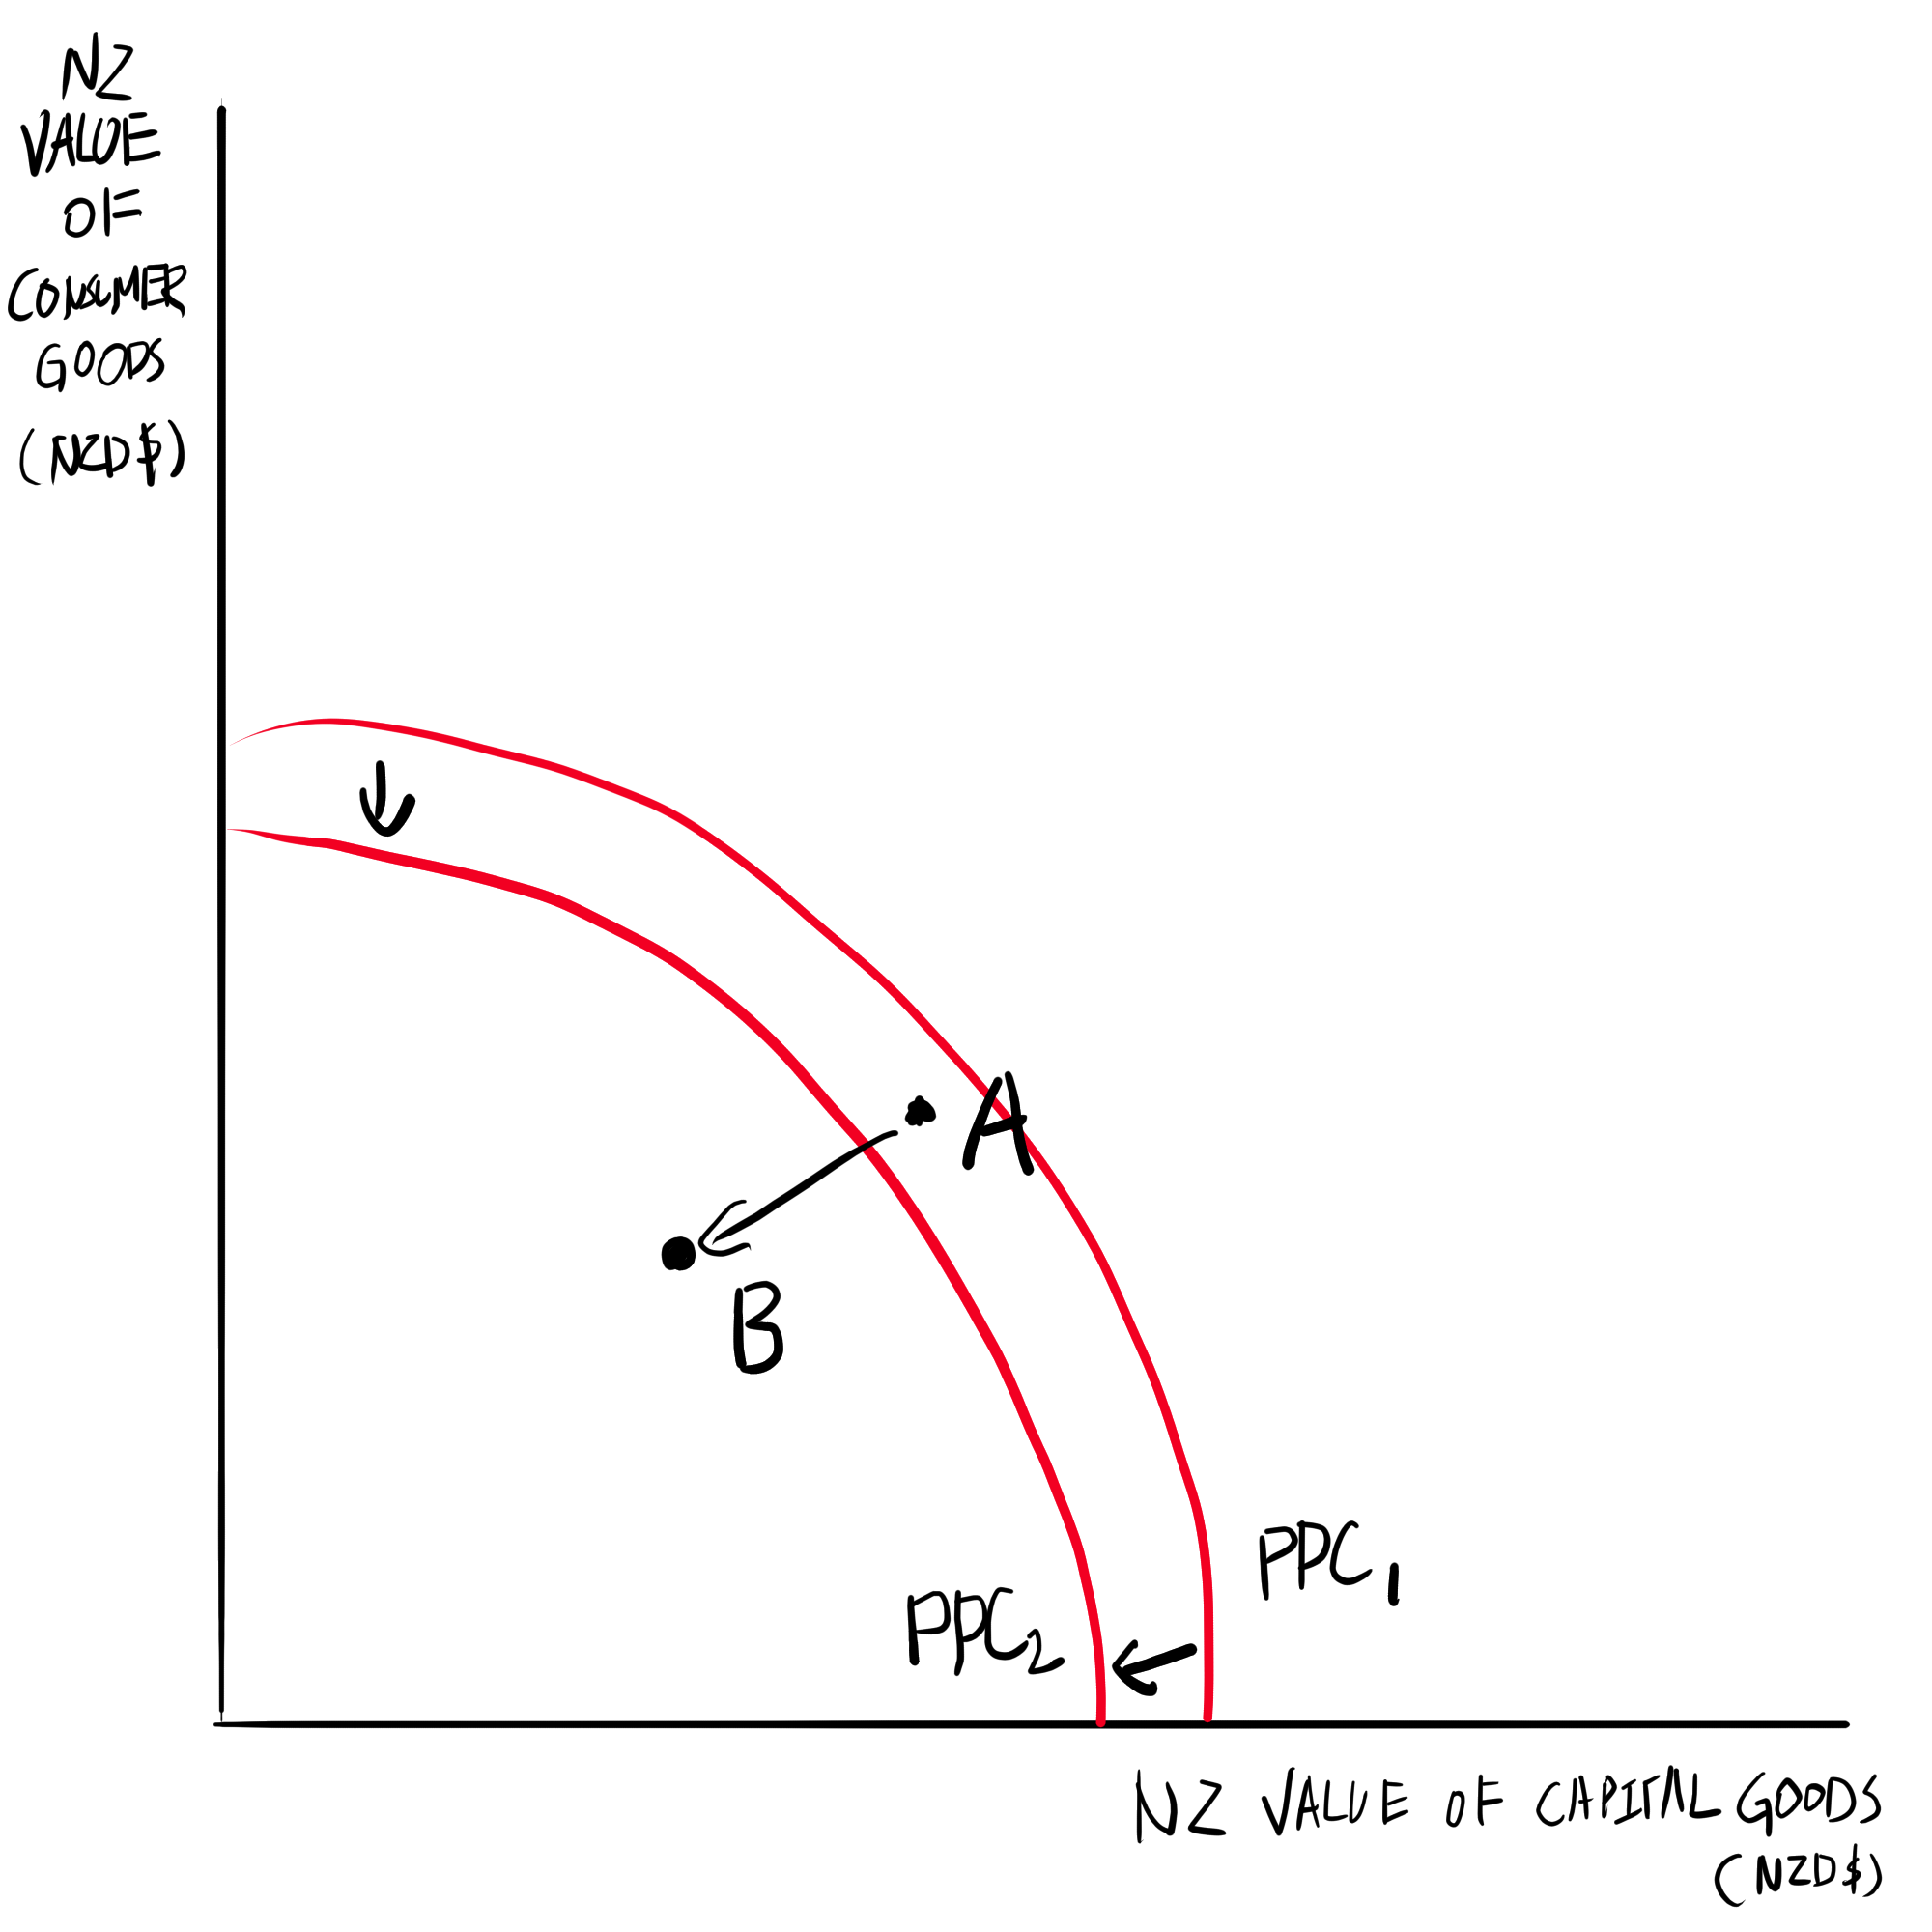
\includegraphics[scale=0.6]{assets/ppf.png}
    \caption{NZ PPF curves during COVID}
    \label{fig:ppf}
\end{figure}

% stakeholders, impacts, ppf
The \textbf{changes} in the AD and AS brings a new economic position within the economy. The decrease in AD creates a recessionary gap, and induces a deflation in the nation which may be desirable for consumers in the short term, as the relative purchasing power of consumers will increase. But due to the interdependence between firms and households, deflation in the long term tends to cause an unemployment investment spiral,
% TODO: explain plz
hurting current debtors and future investors with relatively higher interest rates along the way.
% inflation

% economic growth
Additionally, the decreased economic activity means a lesser efficient economy. Figure \ref{fig:ppf} showcases the \textbf{changes} of NZ's production possibility frontier curve as well as economic positions. The possible short term decrease in the AS is represented from an inwards shift of the PPF curve from $PPC_1$ to $PPC_2$, while the economy position moves from point $A$ to $B$, indicating a fall in the total output of the economy. The most damaging consequence of the negative economic growth is a rise in unemployment.


\section*{Evaluation}
% conclusion, assumptions, short term, priorties, pros and cons

% unemployment
NZ's unemployment rates have steadily increased from the 3rd quarter of 2020 \parencite{unemploy}, as economic theory had predicted. The increased unemployment rates harm the working class both financially and mentally, for the unemployed would receive a lower income, and the need for a job is a common social issue that may increase NZ crime rates in the short term. Both require increasing government expenditure --- in the form of unemployment benefits and policing funds. This reduces public sector spendings on infrastructure. In the retail sector, real life shop owners are likely to be structurally unemployed as the sector endures a structural \textbf{change} towards online shopping. Structural unemployment is a leach on the economy, requiring additional labor force training subsidized by government.

%however
However, the article is optimistic in the ability of the economy to recover. For the pandemic is short term, the release of lockdowns and heavy government stimulus is likely to boost AD, shifting it rightwards. The increase in unemployment, and the fall in AS can be considered to be temporary, for \textbf{changes} caused by the virus will also create new job positions and demands, particularly in the technology sector. Massive government spendings on benefits also serves to increase AD, its effects are boosted through the high propensity of saving of NZ households \parencite{spend}. A swift recovery seems to be expected.

%but: spriral, I ran out of words

\section*{Summary}

% ending
COVID-19 had caused NZ to enter a recession. However, the article and economic theory predicts the impacts of recession to be short termed. Strong and fast government response to the virus seems to guarantee a strong recovery.

\newpage
\nocite{*}
\printbibliography

\end{document}
